\documentclass[11pt]{article}
\usepackage[margin = 1in]{geometry}
\usepackage{amsmath}
\usepackage{amssymb}
\usepackage{amsthm}
\usepackage{graphicx}
\usepackage{subfig}
\usepackage{enumitem}
\usepackage{url}
\usepackage[parfill]{parskip}
\usepackage{listings}
\newcommand{\skipline}{\vspace{\baselineskip}}
\newcommand{\spacer}{\noalign{\medskip}}
\newenvironment{problem}[1]{\textbf{Problem #1: }}{\newpage}


\begin{document}
	
	\begin{center}
		\textbf{Homework 5} \\
		\textbf{Ordinary Differential Equations} \\
		\textbf{Math 537} \\
		\textbf{Stephen Giang RedID: 823184070} \\
		\skipline \skipline
	\end{center}

	\begin{problem}{1}
		Consider the following second-order ordinary differential equations (ODEs) for nonlinear pendulum oscillations:
		\[\frac{d^2\theta}{dt^2} + \epsilon\frac{d\theta}{dt} + \sin(\theta) = 0. \tag{1.1}\]
		Applying Taylor series expansions, Eq. (1.1) can be simplified into one of the
		following systems:
		\[\frac{d^2\theta}{dt^2} + \theta = 0. \tag{1.2} \]
		\[\frac{d^2\theta}{dt^2} + \epsilon\frac{d\theta}{dt} + \theta = 0. \tag{1.3}\]
		\[\frac{d^2\theta}{dt^2} + \left(\theta - \frac{\theta^3}{6}\right) = 0. \tag{1.4}\]
		\begin{enumerate}[label = (\alph*)]
			\item  Perform a linear stability analysis in each of Eqs. (1.2)-(1.4).
			\begin{itemize}
				\item[(1.2) ] We can find the eigenvalues from solving its characteristic equation.
				\[\lambda^2 + 1 = 0\]
				Thus our eigenvalues are $\lambda = \pm i$.  This means that we get a \textbf{Clockwise Center}.
				\item[(1.3) ] We can find the eigenvalues from solving its characteristic equation.
				\[\lambda^2 + \epsilon\lambda + 1 = 0\]
				Thus our eigenvalues are $\lambda = \frac{1}{2}\left(-\epsilon \pm \sqrt{\epsilon^2 - 4}\right)$.
				\\ \\
				For $\epsilon < -2$, we get 2 positive real eigenvalues.  This means that we get an \textbf{Unstable Source}.
				\\ \\
				For $\epsilon = - 2$, we get $\lambda = 1$.  This means that we get an \textbf{Unstable Source}.
				\\ \\
				For $-2 < \epsilon < 0$, we get 2 imaginary eigenvalues with positive real parts.  This means that we get an \textbf{Unstable Spiral}.
				\\ \\
				For $\epsilon = 0$, we get $\lambda = \pm i$.  This means that we get a \textbf{Clockwise Center}.
				\\ \\
				For $0 < \epsilon < 2$, we get 2 imaginary eigenvalues with negative real parts.  This means that we get a \textbf{Stable Spiral}.
				\\ \\
				For $2 < \epsilon$, we get 2 negative real eigenvalues.  This means that we get a \textbf{Stable Sink}.
				\\ \\
				For $\epsilon = 2$, we get $\lambda = -1$.  This means that we get a \textbf{Stable Sink}. 
				\newpage 
				\item[1.4] Let $\phi = \theta'$ and $\phi' = \theta\left(\frac{\theta^2}{6} - 1 \right)$.
				\[X' = \begin{pmatrix}
					\phi \\ \phi'
				\end{pmatrix} = \begin{pmatrix}
					0 & 1 \\ \frac{\theta^2}{6} - 1 & 0
				\end{pmatrix}\begin{pmatrix}
					\theta \\ \phi
				\end{pmatrix} = AX\]
				Notice we can find the critical points:
				\[X' = \begin{pmatrix}
					0 \\ 0
				\end{pmatrix} = \begin{pmatrix}
					0 & 1 \\ \frac{\theta^2}{6} - 1 & 0
				\end{pmatrix}\begin{pmatrix}
					\theta \\ \phi
				\end{pmatrix} = AX\]
				From this we get the following critical points: $(\theta, \phi) = (\pm \sqrt{6},0)$ and $(\theta, \phi) = (0,0)$.
				\\ \\
				Now notice the Jacobian:
				\[J(\theta, \phi) = \left[\begin{array}{cc}
					\frac{d\phi}{d\theta} & \frac{d\phi}{d\theta'} \\
					\spacer \frac{d\phi'}{d\theta} & \frac{d\phi'}{d\theta'}	
				\end{array}\right] = \left[\begin{array}{cc}
					0 & 1 \\ \spacer \frac{\theta^2}{2} - 1 & 0
				\end{array}\right]\]
				Notice the Jacobians and eigenvalues evaluated at the critical points:
				\[J(0,0) = \begin{bmatrix}
					0 & 1 \\ -1 & 0
				\end{bmatrix}\] 
				From solving $|A - \lambda I| = 0$, we get that $\lambda = \pm i$.  Thus we get a \textbf{Clockwise Center}.
				\[J(\pm \sqrt{6}, 0) = \begin{bmatrix}
					0 & 1 \\ 2 & 0
				\end{bmatrix}\]
				From solving $|A - \lambda I| = 0$, we get that $\lambda = \pm \sqrt{2}$.  Thus we get a \textbf{Saddle Point}.
			\end{itemize}
			\skipline
			\item  Discuss the concept of structural stability using results in (1a).
			\\ \\
			Structural Stability is when the linear stability can withstand small changes in perturbation without changing. A linear flow is structurally stable if and only if it is hyperbolic, meaning not having real parts zero.  In (1a): 
			\\ \\
			For equation (1.2), the linear stability was a center so it is \textbf{Structurally Unstable}.  
			\\ \\
			For equation (1.3), the linear stability changed a lot for different values of $\epsilon$.  It was \textbf{Structurally Stable} as long as $\epsilon \not  = 0$.  
			\\ \\
			For equation (1.4), the linear stability was \textbf{Structurally Stable} except at the origin where it was \textbf{Structurally Unstable}
		\end{enumerate}
	\end{problem}

	\begin{problem}{2}
		Consider the following system:
		\[\frac{d^2x}{dt^2} - \alpha x = e^{\beta t}. \tag{2.1}\]
		Complete the following problems with $(\alpha,\beta) = (1,-1)$ and $(\alpha,\beta) = (-1,-1)$
		\begin{enumerate}[label = (\alph*)]
			\item  Solve Eqs. (2.1) for the solutions.
			\begin{enumerate}[label = (\roman*)]
				\item Let $(\alpha,\beta) = (1,-1)$.  Notice we can solve for the homogeneous solution of Eq (2.1).
				\\ \\
				We can find the eigenvalues from solving its characteristic equation.
				\[\lambda^2 - 1 = 0 \qquad \lambda = \pm 1\]
				So we get the homogeneous solution:
				\[x_h = c_1e^{-t} + c_2e^{t}\]
				Using the Method of Undetermined Coefficients, we can try:
				\[x_p = Ae^{- t}t, \qquad x_p' = -Ae^{-t}t + Ae^{-t}, \qquad x_p'' = Ae^{-t}t - 2 Ae^{-t} \]
				Now we can evaluate $y_p$ into Eq (2.1):
				\[Ae^{-t}t - 2Ae^{-t} - Ae^{-t}t = -2 Ae^{-t} = e^{-t}\]
				Thus we get that
				\[A = \frac{-1}{2}\]
				This gives us the solution:
				\[\boldsymbol{x = c_1e^{-t} + c_2e^{t} - \frac{1}{2}te^{-t}}\]
				\item Let $(\alpha,\beta) = (-1,-1)$.  Notice we can solve for the homogeneous solution of Eq (2.1).
				\\ \\
				We can find the eigenvalues from solving its characteristic equation.
				\[\lambda^2 + 1 = 0 \qquad \lambda = \pm i\]
				So we get the homogeneous solution:
				\[x_h = c_1\cos\,t + c_2\sin\,t\]
				Using the Method of Undetermined Coefficients, we can try:
				\[x_p = Ae^{- t}, \qquad x_p' = -Ae^{-t}, \qquad x_p'' = Ae^{-t} \]
				Now we can evaluate $y_p$ into Eq (2.1):
				\[Ae^{-t} + Ae^{-t} = 2 Ae^{-t} = e^{-t}\]
				Thus we get that
				\[A = \frac{1}{2}\]
				This gives us the solution:
				\[\boldsymbol{x = c_1\cos\,t + c_2\sin\,t + \frac{1}{2}e^{-t}}\]
			\end{enumerate}
			\newpage
			\item Convert Eqs. (2.1) into an autonomous linear system which
			consists of three first-order differential equations.
			\\ \\
			Notice we can rewrite the equation as the following:
			\[\frac{d^2x}{dt^2} = \alpha x + e^{\beta t}\]
			Let $u = x'$, $v = e^{\beta t}$ and $w = v' = \beta e^{\beta t}$.  From this we get:
			\[\frac{dx}{dt} = u \qquad \frac{du}{dt} = \alpha x + v \qquad \frac{dv}{dt} = \beta v\]
			Using this we get the system:
			\[\boldsymbol{X' = \begin{pmatrix}
				x' \\ u' \\ v'
			\end{pmatrix} = 
			\begin{pmatrix}
				0 & 1 & 0 \\
				\alpha & 0 & 1 \\
				0 & 0 & \beta
			\end{pmatrix}\begin{pmatrix}
				x \\ u \\ v
			\end{pmatrix} = AX}\]
			\item Solve for the eigenvalues and eigenvectors of the autonomous
			systems in (2b).
			\\ \\
			Notice we can find the eigenvalues from solving $|A - \lambda I| = 0$
			\begin{align*}
				\lambda^2\left(\beta - \lambda\right) - \alpha\left(\beta - \lambda\right) &= 0 & \lambda^2 \left(\lambda - \beta\right) - \alpha\left(\lambda - \beta\right) &= 0 \\
				-\lambda^3 + \beta \lambda^2 + \alpha \lambda - \alpha\beta &= 0 & (\lambda^2 - \alpha)(\lambda - \beta) &= 0\\
				\lambda^3 - \beta \lambda^2 - \alpha \lambda + \alpha\beta &= 0  & \lambda = \pm \sqrt{\alpha}, \beta &\\
			\end{align*}
			For $(\alpha,\beta) = (1,-1)$, we get $\lambda = 1$ and $\lambda = -1$ with multiplicity 2.
			\\ \\
			Notice for $\lambda_1 = 1$, we get the eigenvector: $v_1 = \begin{pmatrix}
				1 \\ 1 \\ 0
			\end{pmatrix}$.
			\\ \\
			Notice for $\lambda_2 = -1$, we get the eigenvector: $v_2 = \begin{pmatrix}
				1 \\ -1 \\ 0
			\end{pmatrix}$.
			\\ \\
			For $\lambda_3 = -1$, we can solve for $v_3$ by solving $|A - \lambda_3|v_3 = v_2$, such that $v_3 = \begin{pmatrix}
				1/2 \\ 1/2 \\ -2
			\end{pmatrix}$
			\newpage
			For $(\alpha,\beta) = (-1,-1)$, we get $\lambda = \pm i$ and $\lambda = -1$.
			\\ \\
			Notice for $\lambda_1 = i$, we get the eigenvector: $v_1 = \begin{pmatrix}
				i \\ 1 \\ 0
			\end{pmatrix}$.
			\\ \\
			Notice for $\lambda_2 = -i$, we get the eigenvector, $v_2$, is just the conjugate of $v_1$, such that : $v_2 = \begin{pmatrix}
				-i \\ 1 \\ 0
			\end{pmatrix}$.
			\\ \\
			For $\lambda_3 = -1$, we get the eigenvector: $v_3 = \begin{pmatrix}
				1/2 \\ -1/2 \\ 1
			\end{pmatrix}$
			\item Compare the results in (2a) and (2c)
			\\ \\
			For $(\alpha,\beta) = (1,-1)$, we get the following solution:
			\[\begin{pmatrix}
				x \\ u \\ v
			\end{pmatrix} = c_1\begin{pmatrix}
				1 \\ 1 \\ 0
			\end{pmatrix}e^t + c_2\begin{pmatrix}
				1 \\ -1	 \\ 0
			\end{pmatrix}e^{-t} + c_3\begin{pmatrix}
				1/2 \\ 1/2 \\ -2
			\end{pmatrix}te^{-t} \]
			\\ \\
			\textbf{Notice the solution for $\boldsymbol{x}$:}
			\[\boldsymbol{x = c_1e^t + c_2e^{-t} + c_3\frac{1}{2}te^{t}}\]
			\textbf{This is the same as part (a) except this has an extra constant $\boldsymbol{c_3}$}. 
			\\ \\
			For $(\alpha,\beta) = (-1,-1)$, we get the following solution:
			\[\begin{pmatrix}
				x \\ u \\ v
			\end{pmatrix} = c_1\begin{pmatrix}
				-\sin\,t \\ \cos\,t \\ 0
			\end{pmatrix} + c_2\begin{pmatrix}
				\cos\,t \\ \sin\,t \\ 0
			\end{pmatrix} + c_3\begin{pmatrix}
				1/2 \\ -1/2 \\ 1
			\end{pmatrix}e^{-t}\]
			\textbf{Notice the solution for $\boldsymbol{x}$:}
			\[\boldsymbol{x = -c_1\sin\,t + c_2\cos\,t + c_3\frac{1}{2}e^{-t}}\]
			\textbf{This is the same as part (a) except this has an extra constant $\boldsymbol{c_3}$}.
		\end{enumerate}
	\end{problem}

	\begin{problem}{3}
		Consider the following coupled harmonic oscillator (as shown
		in Fig. 1):
		\[\frac{d^2x_1}{dt^2} = -k_1x_1 + k_2(x_2 - x_1), \tag{3.1}\]
		\[\frac{d^2x_2}{dt^2} = -k_2(x_2 - x_1). \tag{3.2}\]
		Let $k_1 = 4X^2_c$ and $k_2 = X^2_c$ (and $m_1 = m_2 = 1$).
		\begin{figure}[h!]
			\centering
			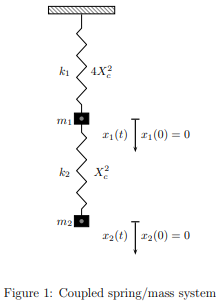
\includegraphics{Prob3}
		\end{figure}
		\begin{enumerate}[label = (\alph*)]
			\item  Convert the above equations into a linear system with first order differential equations.
			\\ \\
			Let $y_1 = x_1'$ and $y_2 = x_2'$.
			\[\boldsymbol{X' = \begin{pmatrix}
				y_1 \\ y_1' \\ y_2 \\ y_2'
			\end{pmatrix} = \begin{pmatrix}
				0 & 1 & 0 & 0 \\
				-5X^2_c & 0 & X^2_c & 0 \\
				0 & 0 & 0 & 1 \\
				X^2_c & 0 & -X^2_c & 0
			\end{pmatrix}\begin{pmatrix}
				x_1 \\ y_1 \\ x_2 \\ y_2
			\end{pmatrix} = AX}\]
			\item  Find the eigenvalues and eigenvectors
			\\ \\
			Notice we can find the eigenvalues from solving $|A - \lambda I| = 0$
			\begin{align*}
				\lambda^2(\lambda^2 + X^2_c) + (5X^2_c)(\lambda^2 + X^2_c) - X^4_c &= 0 \\
				(\lambda^2 + 5X^2_c)(\lambda^2 + X^2_c) - X^4_c &= 0 \\
				\lambda^4 + 6\lambda^2 X^2_c + 4X^4_c &= 0 
			\end{align*}
			From this we get $\lambda_{1,2} = \pm X_c \,i\,\sqrt{3 - \sqrt{5}}$ and $\lambda_{3,4} = \pm X_c \,i\,\sqrt{3 + \sqrt{5}}$
			\newpage
			Notice the eigenvector for $\lambda_1 = X_c\,i\,\sqrt{3 - \sqrt{5}}$:
			\[\begin{pmatrix}
				-X_c\,i\,\sqrt{3 - \sqrt{5}} & 1 & 0 & 0 \\
				-5X^2_c & -X_c\,i\,\sqrt{3 - \sqrt{5}} & X^2_c & 0 \\
				0 & 0 & -X_c\,i\,\sqrt{3 - \sqrt{5}} & 1 \\
				X^2_c & 0 & -X^2_c & -X_c\,i\,\sqrt{3 - \sqrt{5}}
			\end{pmatrix}\begin{pmatrix}
				v_{11} \\ v_{12} \\ v_{13} \\ v_{14}
			\end{pmatrix} = \begin{pmatrix}
				0 \\ 0 \\ 0 \\ 0
			\end{pmatrix} \]
			\[= rref\begin{pmatrix}
				-X_c\,i\,\sqrt{3 - \sqrt{5}} & 1 & 0 & 0 & 0 \\
				-5X^2_c & -X_c\,i\,\sqrt{3 - \sqrt{5}} & X^2_c & 0 & 0 \\
				0 & 0 & -X_c\,i\,\sqrt{3 - \sqrt{5}} & 1 & 0\\
				X^2_c & 0 & -X^2_c & -X_c\,i\,\sqrt{3 - \sqrt{5}} & 0
			\end{pmatrix} \]
			\[= \left(\begin{array}{ccccc}
				1 & 0 & 0 & \frac{\sqrt{2}\,i}{4X_c}\left(3 - \sqrt{5}\right) & 0 \\
				\spacer 0 & 1 & 0 & 2 - \sqrt{5} & 0 \\
				\spacer 0 & 0 & 1 & \frac{\sqrt{2}\,i}{4X_c}\left(1 + \sqrt{5}\right) & 0 \\
				\spacer 0 & 0 & 0 & 0 & 0
			\end{array}\right)\]
			From here, we can let $v_{14} = 1$, such that we get the eigenvector: 
			\[v_1 = \begin{pmatrix}
				v_{11} \\ v_{12} \\ v_{13} \\ v_{14}
			\end{pmatrix} = \left(\begin{array}{c}
				-\frac{\sqrt{2}\,i}{4X_c}\left(3 - \sqrt{5}\right)	\\
				\spacer \sqrt{5} - 2 \\
				\spacer -\frac{\sqrt{2}\,i}{4X_c}\left(1 + \sqrt{5}\right) \\
				\spacer 1
			\end{array}\right)\]
			We can now see that $\lambda_2 = -X_c\,i\,\sqrt{3 - \sqrt{5}}$ is the imaginary conjugate of $\lambda_1$ so we get its eigenvector $v_2$ is the imaginary conjugate of $v_1$:
			\[v_2 = \begin{pmatrix}
				v_{21} \\ v_{22} \\ v_{23} \\ v_{24}
			\end{pmatrix} = \left(\begin{array}{c}
				\frac{\sqrt{2}\,i}{4X_c}\left(3 - \sqrt{5}\right)	\\
				\spacer \sqrt{5} - 2 \\
				\spacer \frac{\sqrt{2}\,i}{4X_c}\left(1 + \sqrt{5}\right) \\
				\spacer 1
			\end{array}\right)\]
			\newpage
			Notice the eigenvector for $\lambda_3 = X_c\,i\,\sqrt{3 + \sqrt{5}}$:
			\[\begin{pmatrix}
				-X_c\,i\,\sqrt{3 + \sqrt{5}} & 1 & 0 & 0 \\
				-5X^2_c & -X_c\,i\,\sqrt{3 + \sqrt{5}} & X^2_c & 0 \\
				0 & 0 & -X_c\,i\,\sqrt{3 + \sqrt{5}} & 1 \\
				X^2_c & 0 & -X^2_c & -X_c\,i\,\sqrt{3 + \sqrt{5}}
			\end{pmatrix}\begin{pmatrix}
				v_{31} \\ v_{32} \\ v_{33} \\ v_{34}
			\end{pmatrix} = \begin{pmatrix}
				0 \\ 0 \\ 0 \\ 0
			\end{pmatrix} \]
			\[= rref\begin{pmatrix}
				-X_c\,i\,\sqrt{3 + \sqrt{5}} & 1 & 0 & 0 & 0 \\
				-5X^2_c & -X_c\,i\,\sqrt{3 + \sqrt{5}} & X^2_c & 0 & 0 \\
				0 & 0 & -X_c\,i\,\sqrt{3 + \sqrt{5}} & 1 & 0\\
				X^2_c & 0 & -X^2_c & -X_c\,i\,\sqrt{3 + \sqrt{5}} & 0
			\end{pmatrix} \]
			\[= \left(\begin{array}{ccccc}
				1 & 0 & 0 & -\frac{\sqrt{2}\,i}{4X_c}\left(3 + \sqrt{5}\right) & 0 \\
				\spacer 0 & 1 & 0 & 2 + \sqrt{5} & 0 \\
				\spacer 0 & 0 & 1 & -\frac{\sqrt{2}\,i}{4X_c}\left(1 - \sqrt{5}\right) & 0 \\
				\spacer 0 & 0 & 0 & 0 & 0
			\end{array}\right)\]
			From here, we can let $v_{34} = 1$, such that we get the eigenvector: 
			\[v_3 = \begin{pmatrix}
				v_{31} \\ v_{32} \\ v_{33} \\ v_{34}
			\end{pmatrix} = \left(\begin{array}{c}
				\frac{\sqrt{2}\,i}{4X_c}\left(3 + \sqrt{5}\right)	\\
				\spacer -\left(2 + \sqrt{5}\right) \\
				\spacer \frac{\sqrt{2}\,i}{4X_c}\left(1 - \sqrt{5}\right) \\
				\spacer 1
			\end{array}\right)\]
			We can now see that $\lambda_4 = -X_c\,i\,\sqrt{3 + \sqrt{5}}$ is the imaginary conjugate of $\lambda_3$ so we get its eigenvector $v_4$ is the imaginary conjugate of $v_3$:
			\[v_4 = \begin{pmatrix}
				v_{41} \\ v_{42} \\ v_{43} \\ v_{44}
			\end{pmatrix} = \left(\begin{array}{c}
				-\frac{\sqrt{2}\,i}{4X_c}\left(3 + \sqrt{5}\right)	\\
				\spacer -\left(2 + \sqrt{5}\right) \\
				\spacer -\frac{\sqrt{2}\,i}{4X_c}\left(1 - \sqrt{5}\right) \\
				\spacer 1
			\end{array}\right)\]
			\newpage
			\item  Find the general solutions.
			\begin{align*}
				\boldsymbol{\begin{pmatrix}
					x_1 \\ y_1 \\ x_2 \\ y_2
				\end{pmatrix}} &\boldsymbol{= c_1\left(\begin{array}{c}
					\frac{\sqrt{2}}{4X_c}\left(3 - \sqrt{5}\right)\sin\left(X_c\sqrt{3 - \sqrt{5}}\,t\right)	\\
					\spacer \left(\sqrt{5} - 2\right)\cos\left(X_c\sqrt{3 - \sqrt{5}}\,t\right) \\
					\spacer \frac{\sqrt{2}}{4X_c}\left(1 + \sqrt{5}\right)\sin\left(X_c\sqrt{3 - \sqrt{5}}\,t\right) \\
					\spacer \cos\left(X_c\sqrt{3 - \sqrt{5}}\,t\right)
				\end{array}\right) + c_2\left(\begin{array}{c}
					-\frac{\sqrt{2}}{4X_c}\left(3 - \sqrt{5}\right)\cos\left(X_c\sqrt{3 - \sqrt{5}}\,t\right)	\\
					\spacer \left(\sqrt{5} - 2\right)\sin\left(X_c\sqrt{3 - \sqrt{5}}\,t\right) \\
					\spacer -\frac{\sqrt{2}}{4X_c}\left(1 + \sqrt{5}\right)\cos\left(X_c\sqrt{3 - \sqrt{5}}\,t\right) \\
					\spacer \sin\left(X_c\sqrt{3 - \sqrt{5}}\,t\right)
				\end{array}\right)} \\
				&\boldsymbol{+ c_3\left(\begin{array}{c}
					-\frac{\sqrt{2}}{4X_c}\left(3 + \sqrt{5}\right)\sin\left(X_c\sqrt{3 + \sqrt{5}}\,t\right)	\\
					\spacer -\left(2 + \sqrt{5}\right)\cos\left(X_c\sqrt{3 + \sqrt{5}}\,t\right) \\
					\spacer -\frac{\sqrt{2}}{4X_c}\left(1 - \sqrt{5}\right)\sin\left(X_c\sqrt{3 + \sqrt{5}}\,t\right) \\
					\spacer \cos\left(X_c\sqrt{3 + \sqrt{5}}\,t\right)
				\end{array}\right) + c_4\left(\begin{array}{c}
					\frac{\sqrt{2}}{4X_c}\left(3 + \sqrt{5}\right)\cos\left(X_c\sqrt{3 + \sqrt{5}}\,t\right)	\\
					\spacer -\left(2 + \sqrt{5}\right)\sin\left(X_c\sqrt{3 + \sqrt{5}}\,t\right) \\
					\spacer \frac{\sqrt{2}}{4X_c}\left(1 - \sqrt{5}\right)\cos\left(X_c\sqrt{3 + \sqrt{5}}\,t\right) \\
					\spacer \sin\left(X_c\sqrt{3 + \sqrt{5}}\,t\right)
				\end{array}\right)}
			\end{align*}
			
		\end{enumerate}
	\end{problem}



\end{document}
